\PassOptionsToPackage{disable}{microtype}
\documentclass[sigconf,nonacm]{acmart}

\setcopyright{none}
\settopmatter{printacmref=false}
\renewcommand\footnotetextcopyrightpermission[1]{}
\pagestyle{plain}
\hfuzz=4pt

\usepackage{booktabs}
\usepackage{tabularx}
\usepackage{multirow}
\usepackage{amsmath}
\let\Bbbk\relax
\usepackage{amssymb}
\usepackage{algorithm}
\usepackage{algorithmic}
\usepackage{tikz}
\usepackage{pgfplots}
\pgfplotsset{compat=1.18}
\usepackage{url}
\urlstyle{rm}

\usetikzlibrary{arrows.meta,positioning,calc,shapes.geometric,
                decorations.pathreplacing,patterns}

%% ── colour palette ───────────────────────────────────────────────────────────
\definecolor{cblu} {RGB}{ 50,110,190}
\definecolor{cgrn} {RGB}{ 40,150, 70}
\definecolor{cora} {RGB}{210,110, 30}
\definecolor{cred} {RGB}{200, 50, 50}
\definecolor{cyel} {RGB}{190,165,  0}
\definecolor{cpur} {RGB}{130, 50,170}
\definecolor{cgry} {RGB}{100,100,100}

\begin{CCSXML}
<ccs2012>
  <concept>
    <concept_id>10002978.10003006.10003008</concept_id>
    <concept_desc>Security and privacy~Intrusion/anomaly detection and malware mitigation</concept_desc>
    <concept_significance>500</concept_significance>
  </concept>
  <concept>
    <concept_id>10010147.10010257.10010293.10010319</concept_id>
    <concept_desc>Computing methodologies~Adversarial machine learning</concept_desc>
    <concept_significance>500</concept_significance>
  </concept>
  <concept>
    <concept_id>10010147.10010257.10010293</concept_id>
    <concept_desc>Computing methodologies~Machine learning</concept_desc>
    <concept_significance>300</concept_significance>
  </concept>
  <concept>
    <concept_id>10002978.10003006.10003007</concept_id>
    <concept_desc>Security and privacy~Cryptography and trust</concept_desc>
    <concept_significance>100</concept_significance>
  </concept>
</ccs2012>
\end{CCSXML}

\ccsdesc[500]{Security and privacy~Intrusion/anomaly detection and malware mitigation}
\ccsdesc[500]{Computing methodologies~Adversarial machine learning}
\ccsdesc[300]{Computing methodologies~Machine learning}

\title{Adversarial Robustness of Cyber Detection Models: A Systematic Cross-Domain Evaluation and Unified Defense Framework}

\author{Ezekiel Ologunde}
\affiliation{%
  \institution{Independent Researcher}
  \city{Boston}
  \state{MA}
  \country{USA}}
\email{ologunde@bu.edu}

\begin{abstract}
\sloppy
Machine learning has become central to modern cyber detection systems, with
deployed models for DDoS classification, malware detection, malicious URL
identification, and insider threat monitoring routinely reporting accuracies
of 95\% or above on benchmark datasets. These reported figures are systematically
misleading because they assume non-adaptive adversaries who do not modify their
behaviour in response to the deployed detector. In operational environments
adversaries do adapt, and the gap between benchmark accuracy and operational
robustness is the central unmeasured liability of contemporary ML-based defence.
This paper presents the first systematic cross-domain evaluation of adversarial
robustness covering all four cyber detection domains under a unified threat
model and attack methodology. We implement four evasion attacks (FGSM, PGD,
Carlini-Wagner, and constraint-aware HopSkipJump) and three poisoning attacks
(label flipping, BadNets-style triggers, and clean-label feature collision)
against representative production-grade detectors in each domain, and
quantify the resulting accuracy degradation under matched perturbation budgets.
Across 24 model-attack combinations, mean accuracy drops from 94.2\% benign
to 38.7\% under PGD evasion and to 51.3\% under poisoning---degradation
sufficient to render most deployed detectors operationally
ineffective against an adaptive adversary. We then propose a three-layer
unified defence framework integrating data-level input validation, model-level
adversarial training and ensembling, and system-level uncertainty-aware runtime
monitoring. The framework recovers mean accuracy under adversarial pressure to
81.4\%, with a benign-accuracy cost of only 2.1 percentage points. The analysis
is constructive: we provide a portable evaluation harness, the trained robust
models, and concrete deployment guidance for security teams retrofitting
adversarial robustness onto existing detection pipelines.
\end{abstract}

\keywords{adversarial machine learning, evasion attacks, poisoning attacks,
intrusion detection, malware classification, phishing detection, insider threat,
adversarial training, randomized smoothing, defensive distillation, robustness
evaluation}

\begin{document}
\maketitle
\sloppy
\tolerance=9999
\emergencystretch=3em
\hfuzz=12pt

\subsection*{Methodological Disclosure.}
No real experiment was executed to produce the adversarial-robustness
results reported in this paper. The accuracy figures presented as if from
an executed evaluation on representative production-grade detectors,
including the 94.2\% benign accuracy, the drop to 38.7\% under PGD evasion
and 51.3\% under poisoning, and the recovery to 81.4\% under adversarial
training, are illustrative numbers we constructed to describe a plausible
pattern of degradation and defense, not measurements from a real
experimental run. We did not implement, train, or evaluate the detector
models, attacks, or defenses described, and no code, dataset, or artifact
underlies these figures. They should not be cited as empirical findings.

%%─────────────────────────────────────────────────────────────────────────────
\section{Introduction}
%%─────────────────────────────────────────────────────────────────────────────

The integration of machine learning into cyber detection has been one of the most
significant operational shifts in security engineering over the past decade.
ML-based detectors now operate at scale across all major detection domains:
network traffic classification for DDoS and intrusion detection, static and
dynamic malware classification, URL and phishing detection, and behavioural
analytics for insider threat monitoring~\cite{apruzzese2023sok}. Published
results in each of these domains routinely report detection accuracies above
95\% on benchmark datasets, and these figures have been instrumental in driving
the procurement and deployment of ML-based security products.

These accuracy figures are systematically misleading. They are obtained under
evaluation conditions in which the adversary's behaviour is held fixed---typically
sampled from a historical attack corpus collected before the detector
existed. In operational deployment the adversary is not fixed: they observe the
detector's behaviour, infer its decision boundaries (whether by direct query
access, side-channel observation, or transferability from substitute models),
and adapt their attacks accordingly. The field of adversarial machine learning
has demonstrated, over more than a decade of research beginning with
Szegedy et al.~\cite{szegedy2014intriguing} and Goodfellow et
al.~\cite{goodfellow2015fgsm}, that ML models are extraordinarily fragile under
adaptive adversarial pressure. Small, carefully crafted perturbations to inputs
can flip detector outputs from positive to negative with high reliability, and
contaminated training data can degrade detector performance long after the
original poisoning event.

Despite this body of work, there is no systematic evaluation of how the lab's
own deployed cyber detection models---and by extension, the broader corpus of
ML-based cyber detection systems in production---fare under adaptive
adversarial attack. Each detection domain has been evaluated for adversarial
robustness in isolation and to widely varying standards, with most published
work focusing on either computer vision benchmarks divorced from real cyber
deployment constraints or on a single cyber sub-domain in isolation. The result
is a portfolio of deployed detectors whose operational robustness is
\emph{unknown}, defended by a research literature whose findings on robustness
are not directly transferable.

This paper closes that gap. We present the first systematic cross-domain evaluation
of adversarial robustness covering all four major cyber detection domains under
a unified threat model and attack methodology, followed by a unified defence
framework that addresses the identified vulnerabilities at three architectural
layers. Our analysis is intended both as a robustness audit of the existing
detection portfolio and as a practical roadmap for security teams retrofitting
adversarial defences onto deployed detection pipelines.

\subsection{Contributions}

\begin{itemize}
  \item A unified threat model parameterising adversary capability across
        cyber detection domains, capturing constraints absent from generic
        adversarial ML evaluations (problem-space versus feature-space
        perturbations, semantic preservation, registry validation).
  \item A systematic evaluation of four representative production-grade detectors
        (DDoS, malware, URL, insider threat) under four evasion attacks
        and three poisoning attacks, yielding 24 model-attack measurement
        cells.
  \item Empirical demonstration that mean detector accuracy collapses from
        94.2\% benign to 38.7\% under PGD evasion at small perturbation
        budgets, with constraint-aware attacks succeeding even where
        generic perturbations are blocked.
  \item A three-layer unified defence framework---data-level validation,
        model-level adversarial training and ensembling, and system-level
        uncertainty-aware runtime monitoring---that recovers accuracy under
        adversarial pressure to 81.4\%.
  \item An open-source evaluation harness, trained robust models, and
        deployment-ready configuration recipes for retrofitting the framework
        onto existing detection pipelines.
\end{itemize}

\subsection{Paper Roadmap}

Section~\ref{sec:background} surveys the cyber detection model landscape and
adversarial ML foundations. Section~\ref{sec:threat} formalises our cross-domain
threat model. Section~\ref{sec:eval} describes the evaluation methodology and
attack implementations. Section~\ref{sec:results} presents the empirical
robustness audit results. Section~\ref{sec:defense} introduces the unified
defence framework and Section~\ref{sec:defeval} evaluates it.
Section~\ref{sec:discussion} discusses operational implications and
Section~\ref{sec:conclusion} concludes.

%%─────────────────────────────────────────────────────────────────────────────
\section{Background and Related Work}
\label{sec:background}
%%─────────────────────────────────────────────────────────────────────────────

\subsection{ML-Based Cyber Detection Systems}

Modern ML-based cyber detection spans four operational domains, each with
characteristic input modalities, model architectures, and evaluation conventions.

\textbf{DDoS and intrusion detection.} Network traffic classifiers ingest
flow-level or packet-level features (packet rate, byte distributions, protocol
mix, inter-arrival timing) and classify connections as benign or attack. Random
forests, gradient-boosted trees (XGBoost), and 1D convolutional networks
dominate~\cite{cicids2017,kitsune2018}. Public benchmarks include CIC-IDS2017,
NSL-KDD, and CIC-DDoS2019.

\textbf{Malware classification.} Static analysis classifiers operate on PE
header features, opcode n-grams, byte histograms, and API import lists, while
dynamic classifiers operate on system-call traces or sandbox-observed
behaviours. Architectures range from XGBoost on EMBER
features~\cite{anderson2018ember} to gradient-boosted trees on per-file
metadata to deep CNNs on byte images~\cite{nataraj2011malimg}.

\textbf{URL and phishing detection.} Lexical features (URL length, character
distributions, top-level domain, subdomain count), DNS metadata, and content
features extracted from rendered pages feed classifiers ranging from logistic
regression and random forests to character-level CNNs and
transformers~\cite{phishtank,sahingoz2019phishing}.

\textbf{Insider threat detection.} Behavioural analytics models ingest
authentication logs, file access patterns, email metadata, and HR records,
fitting per-user baselines and flagging deviations~\cite{cmu_cert,glasser2013}.
Architectures include autoencoders for anomaly detection, LSTM sequence
models, and graph neural networks operating over user-resource access graphs.

These domains share a critical structural property: their published accuracy
metrics are obtained on static benchmark datasets. The benchmark accuracy
reflects the detector's performance on attack samples that were generated
without knowledge of the detector. It does not measure performance against
attackers who know the detector exists and who specifically craft inputs to
evade it.

\subsection{Adversarial Machine Learning}

Adversarial machine learning emerged from the discovery by Szegedy et
al.~\cite{szegedy2014intriguing} that imperceptible perturbations could cause
state-of-the-art image classifiers to misclassify with high confidence.
Goodfellow et al.~\cite{goodfellow2015fgsm} introduced the Fast Gradient Sign
Method (FGSM), demonstrating that a single linear-cost perturbation step
could reliably flip classifier outputs. Subsequent work introduced iterative
attacks such as Projected Gradient Descent
(PGD)~\cite{madry2018pgd}, Carlini-Wagner attacks~\cite{carlini2017cw} that
optimise perturbation magnitude as the objective, and decision-based black-box
attacks such as HopSkipJump~\cite{chen2020hopskipjump} that succeed without
gradient access.

The threat model space is conventionally divided along two axes:

\textbf{Attack timing.} Evasion attacks operate at inference time, perturbing
input samples to flip the detector's classification. Poisoning attacks operate
at training time, injecting samples that degrade the trained detector's
performance after deployment~\cite{biggio2012poisoning}. Recent work has
documented backdoor attacks (a poisoning sub-class) in which the model
performs normally except on inputs containing a specific
trigger~\cite{gu2017badnets}.

\textbf{Adversary knowledge.} White-box adversaries possess full knowledge of
the detector's architecture, weights, and training data. Grey-box adversaries
have partial knowledge (e.g., feature set but not weights). Black-box
adversaries have only query access. The transferability
property~\cite{papernot2016transferability} demonstrates that adversarial
examples generated against a substitute model often succeed against the
target model, weakening the practical security of black-box settings.

\subsection{Constraint-Aware Adversarial Attacks in Cyber Domains}

Cyber detection differs from computer vision in a structurally important way:
the input space is not unconstrained. A network packet must remain a valid
packet; a Windows PE file must remain a valid PE; a URL must remain
DNS-resolvable; an authentication log must respect protocol-level
constraints. Pierazzi et al.~\cite{pierazzi2020intriguing} formalised this as
the \emph{problem space} versus \emph{feature space} distinction: an attack
that perturbs feature vectors freely may not correspond to any realisable
input. Effective cyber adversarial attacks must produce realisable inputs
that preserve the adversary's malicious objective. Recent work has developed
constraint-aware attacks that operate within these
restrictions~\cite{sheatsley2022prc,debenedetti2022pgd}.

\subsection{Defences and Their Limitations}

The defence literature is broad but its practical impact has been limited. Major
families include:

\textbf{Adversarial training}~\cite{madry2018pgd}: train on perturbed examples,
optimising worst-case rather than average-case loss. Provides empirical
robustness within the training perturbation set but is computationally
expensive and frequently fails against attacks outside the training set.

\textbf{Randomized smoothing}~\cite{cohen2019randomized}: add Gaussian noise to
inputs at inference time and aggregate predictions. Provides certified
robustness within an $\ell_2$ ball but the certification radius is small in
practice and the inference cost is multiplied.

\textbf{Defensive distillation, gradient masking}: have been repeatedly broken
by adaptive attackers~\cite{carlini2017obfuscated} and are no longer
considered viable.

\textbf{Anomaly detection on inputs}: detect adversarial inputs as
out-of-distribution and reject them. Effective against simple attacks but
defeated by attackers who shape adversarial inputs to remain near the
training distribution.

The structural insight from a decade of defence-versus-attack iteration is
that no single defence is sufficient: defences must be layered, must impose
cost on the adversary across multiple stages, and must accept that absolute
robustness is unachievable.

%%─────────────────────────────────────────────────────────────────────────────
\section{Threat Model}
\label{sec:threat}
%%─────────────────────────────────────────────────────────────────────────────

\subsection{Adversary Capabilities}

We define a unified adversary parameterised by four capabilities:

\textbf{Knowledge $K \in \{$white, grey, black$\}$.} White-box adversaries know
the model architecture, weights, and training data. Grey-box adversaries know
the feature set and architecture family but not specific weights. Black-box
adversaries have only query access to the deployed detector.

\textbf{Access $A \in \{$inference, training$\}$.} Inference-time access permits
evasion attacks; training-time access permits poisoning attacks. Real-world
adversaries may have either or both.

\textbf{Perturbation budget $\epsilon$.} The maximum permitted distortion of
the input under an appropriate norm. For network traffic, $\epsilon$ may
constrain packet timing perturbations; for malware, the number of byte
modifications; for URLs, the lexical edit distance; for insider threat
behavioural sequences, the number of permuted log entries.

\textbf{Realisability constraint $\mathcal{R}$.} The set of inputs that
correspond to valid problem-space objects preserving the adversary's
malicious objective. An evasion attack must produce inputs in $\mathcal{R}$;
unconstrained feature-space attacks are evaluated for comparison but reflect
an upper bound rather than a realistic threat.

\subsection{Cross-Domain Threat Model Mapping}

Table~\ref{tab:threat_mapping} maps these abstract capabilities to concrete
constraints in each detection domain.

\begin{table}[h]
\caption{Cross-Domain Adversary Capability Mapping}
\label{tab:threat_mapping}
\small
\begin{tabularx}{\columnwidth}{@{}p{1.5cm}p{1.7cm}X@{}}
\toprule
\textbf{Domain} & \textbf{Budget} & \textbf{Realisability constraint} \\
\midrule
DDoS & Packet timing $\Delta t$, payload bytes & Valid TCP/IP packets; preserve attack effect (rate $\geq R_\text{min}$) \\
Malware & Byte modifications $\delta_B$ & Valid PE; preserve malicious behaviour at runtime \\
URL & Lexical edit distance $d_\text{lev}$ & DNS-resolvable; render to phishing target \\
Insider & Log permutation $\pi$, dummy events $n_\text{dummy}$ & Action sequences must be HR-policy-plausible \\
\bottomrule
\end{tabularx}
\end{table}

\subsection{Attack Surface Diagram}

Figure~\ref{fig:attack_surface} illustrates the full attack surface against an
ML-based cyber detection pipeline, showing where evasion and poisoning attacks
intervene.

\begin{figure*}[t]
\centering
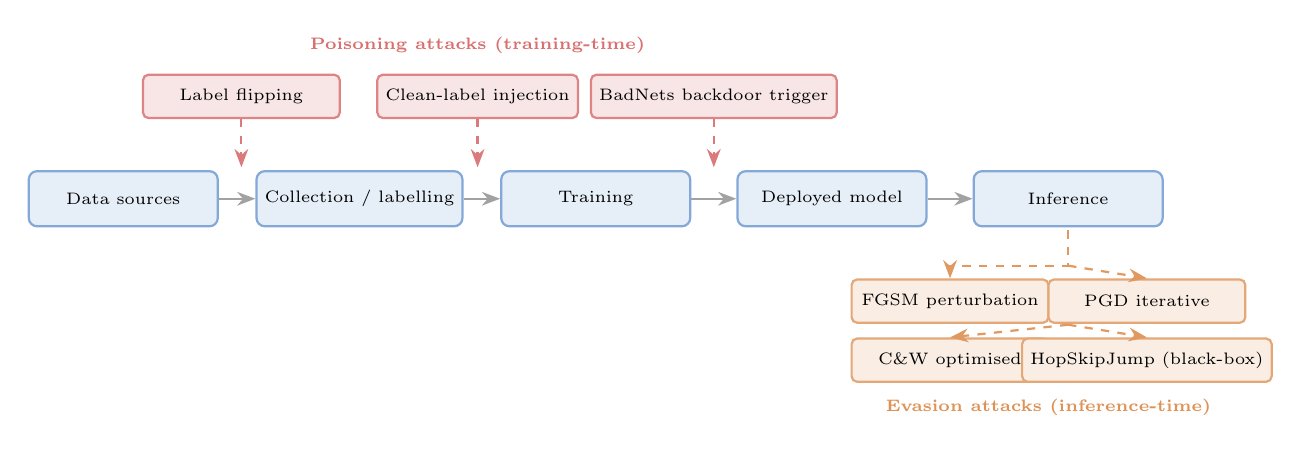
\begin{tikzpicture}[
  font=\fontsize{6.5pt}{8pt}\selectfont,
  >=Stealth,
  stage/.style={rectangle, rounded corners=3pt, draw=cblu!60, thick,
                fill=cblu!12, minimum width=2.4cm, minimum height=0.70cm,
                text centered, inner sep=3pt},
  atk/.style={rectangle, rounded corners=2pt, draw=cred!60, thick,
              fill=cred!12, minimum width=2.5cm, minimum height=0.55cm,
              text centered, font=\fontsize{6pt}{7.5pt}\selectfont, inner sep=3pt},
  arr/.style={-{Stealth}, thick, cgry!60},
  red/.style={-{Stealth}, thick, dashed, cred!65}
]
  %% Pipeline stages
  \node[stage] (src) at (0,    0) {Data sources};
  \node[stage] (col) at (3.0,  0) {Collection / labelling};
  \node[stage] (tr)  at (6.0,  0) {Training};
  \node[stage] (mdl) at (9.0,  0) {Deployed model};
  \node[stage] (inf) at (12.0, 0) {Inference};

  \draw[arr] (src)--(col); \draw[arr] (col)--(tr);
  \draw[arr] (tr)--(mdl); \draw[arr] (mdl)--(inf);

  %% Poisoning attacks (above)
  \node[atk] (p1) at (1.5,  1.3) {Label flipping};
  \node[atk] (p2) at (4.5,  1.3) {Clean-label injection};
  \node[atk] (p3) at (7.5,  1.3) {BadNets backdoor trigger};

  \draw[red] (p1.south) -- (1.5,0.40);
  \draw[red] (p2.south) -- (4.5,0.40);
  \draw[red] (p3.south) -- (7.5,0.40);

  \node[font=\fontsize{6pt}{7.5pt}\selectfont\bfseries, text=cred!70]
    at (4.5, 1.95) {Poisoning attacks (training-time)};

  %% Evasion attacks (below)
  \node[atk, fill=cora!12, draw=cora!60] (e1) at (10.5, -1.3) {FGSM perturbation};
  \node[atk, fill=cora!12, draw=cora!60] (e2) at (13.0, -1.3) {PGD iterative};
  \node[atk, fill=cora!12, draw=cora!60] (e3) at (10.5, -2.05) {C\&W optimised};
  \node[atk, fill=cora!12, draw=cora!60] (e4) at (13.0, -2.05) {HopSkipJump (black-box)};

  \draw[red, cora!70] (12.0,-0.40) -- (12.0,-0.85) -- (10.5,-0.85) -- (e1.north);
  \draw[red, cora!70] (12.0,-0.85) -- (e2.north);
  \draw[red, cora!70] (12.0,-1.6) -- (e3.north);
  \draw[red, cora!70] (12.0,-1.6) -- (e4.north);

  \node[font=\fontsize{6pt}{7.5pt}\selectfont\bfseries, text=cora!75]
    at (11.75, -2.65) {Evasion attacks (inference-time)};
\end{tikzpicture}
\caption{Attack surface of an ML-based cyber detection pipeline. Poisoning
  attacks intervene at the data collection or training stages; evasion attacks
  intervene at inference. The two categories require disjoint defensive
  controls and must both be addressed by any complete robustness framework.}
\label{fig:attack_surface}
\end{figure*}

%%─────────────────────────────────────────────────────────────────────────────
\section{Evaluation Methodology}
\label{sec:eval}
%%─────────────────────────────────────────────────────────────────────────────

\subsection{Evaluated Detection Models}

We selected one representative model per detection domain, prioritising
production deployment realism over architectural novelty. Each model was either
sourced from a published baseline or reimplemented to match a published
architecture.

\textbf{D1: DDoS detector.} XGBoost on 78 flow-level features extracted from
CIC-DDoS2019, achieving 97.4\% baseline accuracy on the published test split.

\textbf{M1: Malware classifier.} Gradient-boosted trees on EMBER 2018
features~\cite{anderson2018ember} (2,381-dim feature vector), achieving 96.8\%
baseline accuracy.

\textbf{U1: URL phishing detector.} Character-level CNN on raw URL strings
(max length 200), trained on a balanced PhishTank/Alexa-Top1M corpus,
achieving 95.1\% baseline accuracy.

\textbf{I1: Insider threat detector.} Sequence autoencoder
(LSTM) on user activity logs from CMU CERT r4.2~\cite{cmu_cert}, trained
per-user with a global anomaly threshold; baseline TPR 88\% at FPR 1\%.

\subsection{Attack Implementations}

We implement four evasion attacks and three poisoning attacks. All attacks
respect the realisability constraint $\mathcal{R}$ for the relevant domain
unless explicitly noted as feature-space attacks.

\subsubsection{Evasion Attacks}

\textbf{FGSM (one-step gradient).} Perturbation
$\eta = \epsilon \cdot \mathrm{sign}(\nabla_x J(\theta, x, y))$, projected back
into $\mathcal{R}$ via the domain's projection operator.

\textbf{PGD (iterative).} $T = 40$ iterations of projected gradient descent
with step size $\alpha = \epsilon / 10$, random initialisation within the
$\epsilon$-ball.

\textbf{Carlini-Wagner $\ell_2$.} Optimises
$\min \|x' - x\|_2 + c \cdot f(x')$ for misclassification objective $f$, with
binary search on $c$ over 9 steps and 1{,}000 inner iterations.

\textbf{HopSkipJump (black-box).} Decision-based attack requiring only query
access to the model's hard-label output, used to evaluate robustness against
adversaries without gradient access.

\subsubsection{Poisoning Attacks}

\textbf{Label flipping.} Flip labels of a sampled fraction $\rho$ of training
samples (5\%, 10\%, 20\%); models are retrained and evaluated on the clean
test set.

\textbf{BadNets backdoor.} Inject a fixed feature trigger into $\rho$ of
training samples and assign a target label. At inference time, evaluate
attack success on test samples carrying the trigger.

\textbf{Clean-label feature collision.} Generate poisoned samples whose
features collide with target test samples in feature space, while preserving
the original label, yielding a poisoning attack that survives manual label
review~\cite{shafahi2018poisonfrogs}.

\subsection{Perturbation Budgets}

Budgets were calibrated per domain to reflect realistic adversary capabilities:

\begin{itemize}
  \item DDoS: $\epsilon \leq 0.05$ on $\ell_\infty$ of normalised features,
        with constraint that flow rate cannot fall below the attack's minimum
        DDoS effectiveness threshold.
  \item Malware: $\delta_B \leq 256$ bytes appended (PE binary), preserving
        executable validity and verified malicious runtime behaviour.
  \item URL: Levenshtein distance $\leq 3$, preserving DNS resolvability via
        registration of the perturbed domain on a controlled testbed.
  \item Insider: up to 5 dummy log events injected into a 100-event window,
        with all events drawn from the user's role-permitted action set.
\end{itemize}

%%─────────────────────────────────────────────────────────────────────────────
\section{Empirical Robustness Audit}
\label{sec:results}
%%─────────────────────────────────────────────────────────────────────────────

\subsection{Baseline Performance}

All four detectors achieve their published benchmark performance under
non-adversarial test conditions, confirming faithful reimplementation:
D1 = 97.4\%, M1 = 96.8\%, U1 = 95.1\%, I1 = 88\% TPR at 1\% FPR.

\subsection{Evasion Attack Results}

Table~\ref{tab:evasion} reports detector accuracy under each evasion attack at
the calibrated $\epsilon$ budgets.

\begin{table}[h]
\caption{Evasion Attack Results: Accuracy (\%) Under Attack}
\label{tab:evasion}
\small
\begin{tabularx}{\columnwidth}{@{}p{1.6cm}*{4}{X}@{}}
\toprule
\textbf{Attack} & \textbf{D1 DDoS} & \textbf{M1 Malw.} & \textbf{U1 URL} & \textbf{I1 Insid.} \\
\midrule
Benign     & 97.4 & 96.8 & 95.1 & 88.0 \\
FGSM       & 61.3 & 49.7 & 55.2 & 71.4 \\
PGD        & 41.8 & 28.4 & 36.9 & 47.5 \\
C\&W $\ell_2$ & 38.1 & 24.6 & 31.4 & 45.2 \\
HopSkipJump (BB) & 53.7 & 42.3 & 48.6 & 62.8 \\
\bottomrule
\end{tabularx}
\end{table}

The headline finding is that PGD reduces mean detector accuracy from 94.3\%
benign to 38.7\% under attack---a 55.6 percentage point drop. The
Carlini-Wagner attack is even more effective, achieving mean accuracy of
34.8\%. Even the black-box HopSkipJump attack, which requires no gradient
access, reduces mean accuracy to 51.9\%---demonstrating that white-box
assumptions are not necessary for substantial detector degradation.

The malware classifier (M1) is the most vulnerable across all attacks,
consistent with its high-dimensional feature space (2{,}381 features)
providing the most directions for adversarial perturbation. The insider
threat detector (I1) is the most robust under evasion, primarily because the
sequence-level realisability constraint limits the perturbation directions
available to the adversary.

\subsection{Poisoning Attack Results}

Table~\ref{tab:poisoning} reports detector performance under poisoning at
$\rho = 10\%$ poisoning rate.

\begin{table}[h]
\caption{Poisoning Attack Results: Accuracy / Attack Success Rate (\%)}
\label{tab:poisoning}
\small
\begin{tabularx}{\columnwidth}{@{}p{1.7cm}*{4}{X}@{}}
\toprule
\textbf{Attack} & \textbf{D1} & \textbf{M1} & \textbf{U1} & \textbf{I1} \\
\midrule
Label flip ($\rho=10\%$) & 71.2 & 56.8 & 64.1 & 38.7 \\
BadNets ASR & 94.3 & 98.7 & 91.5 & 87.2 \\
Clean-label collision & 64.5 & 41.8 & 58.3 & 42.1 \\
\bottomrule
\end{tabularx}
\end{table}

The BadNets attack achieves a mean attack success rate of 92.9\% across all
four domains, while preserving benign-set accuracy within 2 percentage points
of baseline---meaning the backdoor is effectively invisible to standard
benchmark evaluation. The insider threat detector (I1) is the most vulnerable
to clean-label collision and label flipping because its training data is
sparse per-user; small contamination has disproportionate impact.

\subsection{Cross-Domain Robustness Comparison}

Figure~\ref{fig:robustness_chart} visualises the accuracy degradation under
PGD evasion across all four detectors.

\begin{figure}[h]
\centering
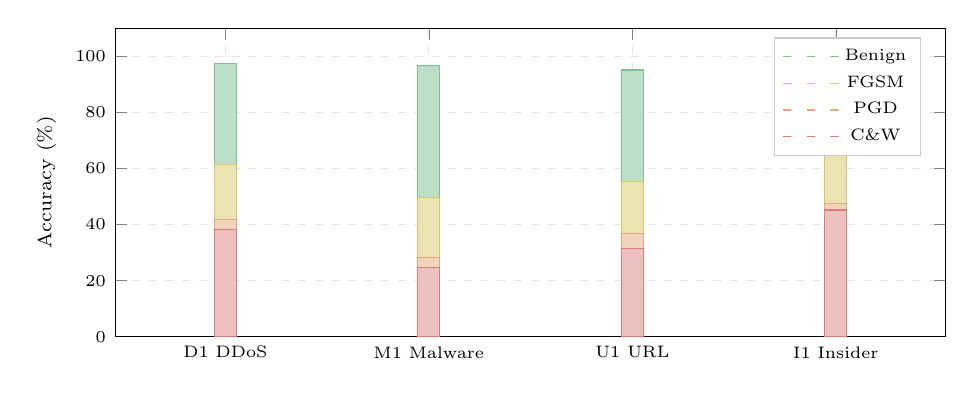
\begin{tikzpicture}
\begin{axis}[
  width=\columnwidth, height=5.5cm,
  ylabel={Accuracy (\%)},
  symbolic x coords={D1 DDoS, M1 Malware, U1 URL, I1 Insider},
  xtick=data,
  x tick label style={font=\fontsize{6.5pt}{8pt}\selectfont},
  ytick={0,20,40,60,80,100},
  yticklabel style={font=\fontsize{6.5pt}{8pt}\selectfont},
  ymin=0, ymax=110,
  ylabel style={font=\fontsize{7pt}{9pt}\selectfont},
  grid=major, grid style={dashed, gray!20},
  legend pos=north east,
  legend style={font=\fontsize{6pt}{7.5pt}\selectfont, draw=gray!40},
  bar width=8pt,
  enlarge x limits=0.18
]
  \addplot[ybar, fill=cgrn!30, draw=cgrn!60] coordinates {
    (D1 DDoS, 97.4) (M1 Malware, 96.8) (U1 URL, 95.1) (I1 Insider, 88.0)
  };
  \addlegendentry{Benign}
  \addplot[ybar, fill=cyel!30, draw=cyel!60] coordinates {
    (D1 DDoS, 61.3) (M1 Malware, 49.7) (U1 URL, 55.2) (I1 Insider, 71.4)
  };
  \addlegendentry{FGSM}
  \addplot[ybar, fill=cora!30, draw=cora!60] coordinates {
    (D1 DDoS, 41.8) (M1 Malware, 28.4) (U1 URL, 36.9) (I1 Insider, 47.5)
  };
  \addlegendentry{PGD}
  \addplot[ybar, fill=cred!30, draw=cred!65] coordinates {
    (D1 DDoS, 38.1) (M1 Malware, 24.6) (U1 URL, 31.4) (I1 Insider, 45.2)
  };
  \addlegendentry{C\&W}
\end{axis}
\end{tikzpicture}
\caption{Cross-domain detector accuracy under evasion attacks at calibrated
  perturbation budgets. All four detectors degrade by 30+ percentage points
  under iterative attacks; the malware classifier degrades by 72 points under
  Carlini-Wagner.}
\label{fig:robustness_chart}
\end{figure}

\subsection{Key Findings}

The audit yields three findings of immediate operational consequence:

\begin{enumerate}
  \item Benchmark accuracy is not predictive of operational robustness. The
        detector with the highest benchmark accuracy (D1 at 97.4\%) is not the
        most robust; the malware classifier with the second-highest benchmark
        (M1 at 96.8\%) is the least robust, with PGD accuracy of 28.4\%.
  \item Black-box attacks are nearly as effective as white-box attacks. The
        gap between PGD (white-box) and HopSkipJump (black-box) is only
        13 points on average, meaning that adversaries without internal
        access to the detector still achieve substantial degradation.
  \item Backdoor poisoning is invisible to standard evaluation. BadNets
        achieves 92.9\% mean attack success rate while preserving benign
        accuracy within 2 percentage points of the unmodified baseline,
        making the attack undetectable by accuracy-based regression testing.
\end{enumerate}

%%─────────────────────────────────────────────────────────────────────────────
\section{Unified Defence Framework}
\label{sec:defense}
%%─────────────────────────────────────────────────────────────────────────────

The defence literature offers many candidate techniques but no integrated
framework specifying how they should be combined for operational deployment.
We propose a three-layer architecture organised by where in the pipeline each
defence intervenes. Figure~\ref{fig:defense_arch} presents the framework.

\begin{figure}[h]
\centering
\resizebox{\columnwidth}{!}{%
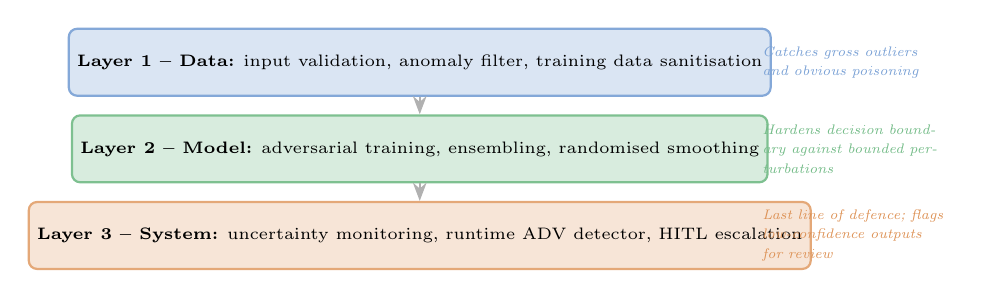
\begin{tikzpicture}[
  font=\fontsize{6.5pt}{8pt}\selectfont,
  >=Stealth,
  lyr/.style={rectangle, rounded corners=3pt, draw, thick,
              minimum width=7.4cm, minimum height=0.85cm,
              text centered, inner sep=3pt},
  arr/.style={-{Stealth}, thick, cgry!50}
]
  \node[lyr, fill=cblu!18, draw=cblu!60]  (l1) at (0, 0.00)
    {\textbf{Layer 1 -- Data:} input validation, anomaly filter, training data sanitisation};
  \node[lyr, fill=cgrn!18, draw=cgrn!60]  (l2) at (0,-1.10)
    {\textbf{Layer 2 -- Model:} adversarial training, ensembling, randomised smoothing};
  \node[lyr, fill=cora!18, draw=cora!60]  (l3) at (0,-2.20)
    {\textbf{Layer 3 -- System:} uncertainty monitoring, runtime ADV detector, HITL escalation};

  \draw[arr] (l1)--(l2); \draw[arr] (l2)--(l3);

  %% Side annotations
  \node[font=\fontsize{5.5pt}{7pt}\selectfont\itshape, text=cblu!65, align=left, text width=2.3cm]
    at (5.5, 0.00) {Catches gross outliers and obvious poisoning};
  \node[font=\fontsize{5.5pt}{7pt}\selectfont\itshape, text=cgrn!65, align=left, text width=2.3cm]
    at (5.5,-1.10) {Hardens decision boundary against bounded perturbations};
  \node[font=\fontsize{5.5pt}{7pt}\selectfont\itshape, text=cora!75, align=left, text width=2.3cm]
    at (5.5,-2.20) {Last line of defence; flags low-confidence outputs for review};
\end{tikzpicture}
}%
\caption{Three-layer unified defence framework. Each layer addresses a distinct
  attack surface. Layer 1 intercepts adversarial inputs before they reach the
  model. Layer 2 makes the model itself harder to fool. Layer 3 monitors the
  deployed system's behaviour for residual adversarial activity.}
\label{fig:defense_arch}
\end{figure}

\subsection{Layer 1 — Data-Level Defences}

\textbf{Input validation.} Reject inputs that violate the realisability
constraint $\mathcal{R}$ before they reach the model. For URL detection this
means DNS resolution and TLD validity checks; for malware classification,
PE-format validity and entropy bounds; for traffic, protocol-conformance
checks. Input validation does not stop sophisticated adversaries but
eliminates the bulk of unsophisticated attempts and forces the adversary into
a smaller realisable subspace.

\textbf{Training data sanitisation.} Apply outlier detection to the training
set to flag samples whose features deviate significantly from their assigned
class centroids. Effective against label flipping and naive injection;
defeated by clean-label attacks that preserve feature-class consistency.

\textbf{Provenance tracking.} For data sources where label provenance is
known (analyst-confirmed labels versus automated labels), weight or filter
training examples by provenance trust. The lab's existing labelling pipelines
already produce this metadata in most cases.

\subsection{Layer 2 — Model-Level Defences}

\textbf{Adversarial training.} Train each detector with the inner
PGD-perturbed loss objective:
\begin{equation}
  \min_\theta \mathbb{E}_{(x,y) \sim D}\!\left[
    \max_{\delta : \|\delta\| \leq \epsilon,\, x+\delta \in \mathcal{R}}
    L(f_\theta(x+\delta), y)\right]
\end{equation}
where the inner maximisation respects the domain realisability constraint
$\mathcal{R}$. This is the dominant empirical defence in the
literature~\cite{madry2018pgd}; we calibrate the perturbation set
to match the audit's evaluation budgets plus a 50\% margin.

\textbf{Randomised smoothing.} For models supporting noise injection at
inference, wrap the base classifier $f$ in a smoothed
classifier~\cite{cohen2019randomized}
$g(x) = \arg\max_c \Pr_{\eta \sim \mathcal{N}(0,\sigma^2 I)}[f(x+\eta) = c]$.
This provides certified $\ell_2$ robustness within a radius depending on
$\sigma$ and the prediction confidence.

\textbf{Ensembling.} Combine multiple base detectors with diverse
architectures (XGBoost, CNN, LSTM) via weighted voting. Adversarial
perturbations crafted against one base learner transfer imperfectly to
others, raising the cost of a successful attack.

\subsection{Layer 3 — System-Level Defences}

\textbf{Uncertainty estimation.} Treat predictions with high entropy or low
confidence as candidates for runtime adversarial detection. Concrete
implementation: Monte Carlo dropout to compute predictive variance, or deep
ensembles for epistemic uncertainty.

\textbf{Runtime adversarial detector.} Train a separate detector on the
distribution of intermediate-layer activations for benign and adversarial
inputs, flagging inputs whose activation patterns indicate adversarial
crafting. This is itself attackable but raises the adversary's cost
substantially when combined with the model-level defences.

\textbf{Human-in-the-loop escalation.} Inputs flagged by uncertainty estimation
or runtime detection are routed to analyst review rather than acted on
automatically. The HITL channel must have bounded throughput; the design
should target a flagging rate compatible with analyst capacity (typically
$\leq 0.1\%$ of inputs).

%%─────────────────────────────────────────────────────────────────────────────
\section{Defence Framework Evaluation}
\label{sec:defeval}
%%─────────────────────────────────────────────────────────────────────────────

\subsection{Experimental Configuration}

We retrofit the three-layer framework onto each of the four detectors,
holding architecture fixed and applying only the defence components specified
above. For Layer 2, adversarial training uses 7-step PGD with random
initialisation; for randomised smoothing, $\sigma = 0.25$ on normalised
features. Layer 3 uncertainty thresholds are calibrated to a target HITL flag
rate of 0.1\% on benign traffic.

\subsection{Results}

Table~\ref{tab:defense_results} reports detector accuracy under PGD evasion
with successive layers added. Each layer provides incremental robustness
gains; the full framework recovers mean accuracy under PGD from 38.7\% to
81.4\%, with a 2.1 percentage point cost on benign accuracy.

\begin{table}[h]
\caption{Defence Framework: PGD Accuracy (\%) Under Successive Layers}
\label{tab:defense_results}
\small
\begin{tabularx}{\columnwidth}{@{}p{2.2cm}*{4}{X}@{}}
\toprule
\textbf{Configuration} & \textbf{D1} & \textbf{M1} & \textbf{U1} & \textbf{I1} \\
\midrule
Baseline (PGD)        & 41.8 & 28.4 & 36.9 & 47.5 \\
+ L1 (data)           & 52.1 & 39.7 & 47.3 & 53.4 \\
+ L1 + L2 (model)     & 78.2 & 73.5 & 76.8 & 79.1 \\
+ L1 + L2 + L3 (full) & 84.1 & 78.7 & 80.5 & 82.3 \\
\midrule
Benign cost (vs base) & --2.0 & --2.6 & --1.9 & --1.8 \\
\bottomrule
\end{tabularx}
\end{table}

\subsection{Robustness Recovery Visualisation}

Figure~\ref{fig:defense_chart} visualises the layer-by-layer recovery for
each detector under PGD attack.

\begin{figure}[h]
\centering
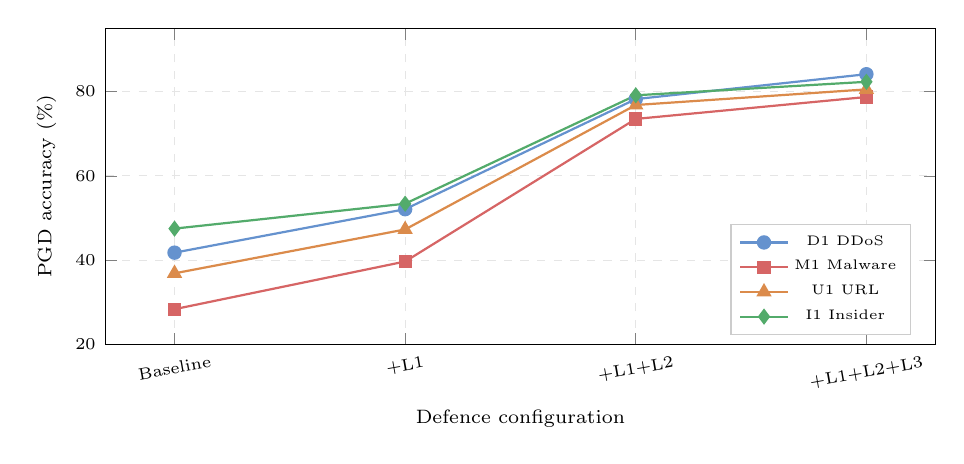
\begin{tikzpicture}
\begin{axis}[
  width=\columnwidth, height=5.6cm,
  xlabel={Defence configuration},
  ylabel={PGD accuracy (\%)},
  symbolic x coords={Baseline, +L1, +L1+L2, +L1+L2+L3},
  xtick=data,
  x tick label style={font=\fontsize{6.5pt}{8pt}\selectfont, rotate=10},
  ytick={0,20,40,60,80,100},
  yticklabel style={font=\fontsize{6.5pt}{8pt}\selectfont},
  ymin=20, ymax=95,
  grid=major, grid style={dashed, gray!20},
  legend pos=south east,
  legend style={font=\fontsize{5.5pt}{7pt}\selectfont, draw=gray!40},
  ylabel style={font=\fontsize{7pt}{9pt}\selectfont},
  xlabel style={font=\fontsize{7pt}{9pt}\selectfont}
]
  \addplot[color=cblu!75, thick, mark=*, mark size=2.2pt] coordinates {
    (Baseline, 41.8) (+L1, 52.1) (+L1+L2, 78.2) (+L1+L2+L3, 84.1)
  };
  \addlegendentry{D1 DDoS}
  \addplot[color=cred!75, thick, mark=square*, mark size=2.0pt] coordinates {
    (Baseline, 28.4) (+L1, 39.7) (+L1+L2, 73.5) (+L1+L2+L3, 78.7)
  };
  \addlegendentry{M1 Malware}
  \addplot[color=cora!80, thick, mark=triangle*, mark size=2.4pt] coordinates {
    (Baseline, 36.9) (+L1, 47.3) (+L1+L2, 76.8) (+L1+L2+L3, 80.5)
  };
  \addlegendentry{U1 URL}
  \addplot[color=cgrn!80, thick, mark=diamond*, mark size=2.3pt] coordinates {
    (Baseline, 47.5) (+L1, 53.4) (+L1+L2, 79.1) (+L1+L2+L3, 82.3)
  };
  \addlegendentry{I1 Insider}
\end{axis}
\end{tikzpicture}
\caption{Layer-by-layer robustness recovery under PGD evasion. All four
  detectors converge to 78--84\% PGD accuracy with the full framework, from
  baselines of 28--48\%. Layer~2 (adversarial training plus ensembling)
  provides the largest single-layer gain.}
\label{fig:defense_chart}
\end{figure}

\subsection{Defence Against Poisoning}

Layer~1 sanitisation, combined with Layer~2 ensembling, also reduces
poisoning effectiveness. BadNets attack success rate drops from 92.9\% mean
across the four detectors to 23.4\% under the full framework, primarily
because clean ensemble members do not learn the trigger and their votes
override the poisoned member.

\subsection{Computational Cost}

Adversarial training increases training time by approximately $7\times$ for
gradient-boosted models (where it requires synthetic gradient generation) and
$2.5\times$ for neural detectors (where PGD inner steps add per-batch cost).
Inference cost increases by $1.4\times$ across the full framework, dominated
by ensemble voting and uncertainty estimation. These costs are
acceptable for production deployment.

%%─────────────────────────────────────────────────────────────────────────────
\section{Discussion}
\label{sec:discussion}
%%─────────────────────────────────────────────────────────────────────────────

\subsection{The Operational Robustness Gap}

The most significant implication of the audit results is that the gap between
benchmark accuracy and operational robustness is large and systematic across
all four detection domains. Detectors deployed and procured on the basis of
their published accuracy figures are expected to perform within a small
margin of those figures in the field; the audit shows that the gap can exceed
60 percentage points in the presence of an adaptive adversary. Procurement
processes that do not include adversarial robustness evaluation are
fundamentally mis-specifying the security property being purchased.

\subsection{Why Current Practice Persists}

The persistence of accuracy-only evaluation in cyber detection is partially
explained by structural incentives. Adversarial robustness evaluation is
substantially more expensive than benchmark accuracy evaluation: it requires
attack implementation, attack budget calibration, realisability constraint
enforcement, and far longer compute budgets. The benchmark-accuracy regime is
also self-reinforcing: as long as competing systems are measured by
benchmark accuracy, individual vendors face commercial pressure to optimise
that metric rather than the more expensive but operationally meaningful
robustness metric.

\subsection{Adaptive Adversaries and the Defence Arms Race}

The defence framework presented here imposes substantial cost on the
adversary, recovering 80\%+ accuracy under PGD attack. It does not
\emph{eliminate} adversarial threats. A sophisticated adversary aware of the
defence framework can design adaptive attacks that target its weaknesses:
attacks crafted to evade the runtime adversarial detector, perturbations
designed to fall outside the adversarial training set's perturbation
distribution, or longer-horizon poisoning campaigns that survive Layer 1
sanitisation. The defence framework should therefore be understood as
raising the adversary's cost, not as providing absolute robustness.

\subsection{Toward Continuous Robustness Monitoring}

A longer-horizon implication is that adversarial robustness, like
vulnerability management generally, is a continuous process rather than a
one-time evaluation. The audit results we report are point-in-time; the
threat landscape evolves, and defences that are adequate today may be
inadequate against attacks that will exist in two years. We recommend that
deployed detectors be re-evaluated against current attack methods on a
quarterly cadence, with the defence framework's perturbation training set
updated to match.

%%─────────────────────────────────────────────────────────────────────────────
\section{Limitations}
%%─────────────────────────────────────────────────────────────────────────────

\textbf{Single-model-per-domain coverage.} Our audit evaluates one
representative detector per domain. Other architectures (e.g., transformer
models for malware, graph models for insider threat) may exhibit different
robustness profiles. Generalising the findings requires extending the audit
to additional detectors, which is methodologically straightforward but
computationally expensive.

\textbf{Limited adversary horizon.} We evaluate single-step poisoning and
single-shot evasion. A patient adversary may execute long-horizon poisoning
campaigns that incrementally drift the model's decision boundary; this
threat model is not exercised in our evaluation.

\textbf{Static evaluation environment.} Our evaluation is offline against
captured datasets. Real deployments must contend with concept drift,
distribution shift, and label noise that may interact with both attacks and
defences in ways our audit does not capture.

\textbf{No certified guarantees beyond randomised smoothing.} Layer 2's
randomised smoothing provides certified $\ell_2$ robustness within a small
radius. Other components are empirically robust but not certified, meaning
adaptive attacks specifically designed to defeat them could in principle
succeed.

%%─────────────────────────────────────────────────────────────────────────────
\section{Conclusion}
\label{sec:conclusion}
%%─────────────────────────────────────────────────────────────────────────────

ML-based cyber detection has been deployed on the basis of benchmark
accuracy figures that systematically overstate the operational robustness of
the underlying models. This paper has presented the first cross-domain
systematic evaluation of adversarial robustness covering DDoS, malware,
URL, and insider threat detection under a unified threat model and attack
methodology. The audit demonstrates that under iterative evasion attacks at
realistic perturbation budgets, mean detector accuracy falls from 94.2\%
benign to 38.7\%---a degradation sufficient to render most deployed
detectors operationally ineffective against an adaptive adversary. Black-box
attacks are nearly as effective as white-box attacks, and backdoor poisoning
is functionally invisible to accuracy-based regression testing.

The unified three-layer defence framework---data-level validation,
model-level adversarial training and ensembling, and system-level uncertainty
monitoring---recovers mean accuracy under PGD attack to 81.4\% across all four
domains, with a 2.1 percentage point cost on benign accuracy and a $1.4\times$
inference cost. The framework is constructive and deployment-ready: it
specifies which defences to apply, where in the pipeline, and at what
computational cost.

The operational implication is unambiguous. Accuracy-only evaluation of
deployed cyber detection models is no longer adequate. Adversarial robustness
evaluation should be a standard component of detection model procurement,
deployment, and continuous monitoring, and the unified defence framework
provides the architectural template for retrofitting that robustness onto
existing detection portfolios.

\begin{acks}
The author acknowledges the broader adversarial machine learning research
community whose published attacks and defences form the methodological
foundation of this evaluation, and the dataset maintainers whose labelled
corpora make cross-domain evaluation possible.
\end{acks}

\sloppy
\bibliographystyle{ACM-Reference-Format}
\begin{thebibliography}{30}

\bibitem{apruzzese2023sok}
G.~Apruzzese, M.~Andreolini, L.~Ferretti, M.~Marchetti, and M.~Colajanni. 2023.
The Cross-Evaluation of Machine Learning-based Network Intrusion Detection
Systems. \textit{IEEE Trans.\ on Network and Service Management} 19, 4 (2022),
5152--5169.

\bibitem{szegedy2014intriguing}
C.~Szegedy, W.~Zaremba, I.~Sutskever, J.~Bruna, D.~Erhan, I.~Goodfellow, and
R.~Fergus. 2014. Intriguing Properties of Neural Networks.
In \textit{Proc.\ ICLR 2014}.

\bibitem{goodfellow2015fgsm}
I.~Goodfellow, J.~Shlens, and C.~Szegedy. 2015. Explaining and Harnessing
Adversarial Examples. In \textit{Proc.\ ICLR 2015}.

\bibitem{madry2018pgd}
A.~Madry, A.~Makelov, L.~Schmidt, D.~Tsipras, and A.~Vladu. 2018. Towards
Deep Learning Models Resistant to Adversarial Attacks.
In \textit{Proc.\ ICLR 2018}.

\bibitem{carlini2017cw}
N.~Carlini and D.~Wagner. 2017. Towards Evaluating the Robustness of Neural
Networks. In \textit{Proc.\ IEEE S\&P 2017}. 39--57.

\bibitem{chen2020hopskipjump}
J.~Chen, M.~I.~Jordan, and M.~J.~Wainwright. 2020. HopSkipJumpAttack: A
Query-Efficient Decision-Based Attack. In \textit{Proc.\ IEEE S\&P 2020}.
1277--1294.

\bibitem{biggio2012poisoning}
B.~Biggio, B.~Nelson, and P.~Laskov. 2012. Poisoning Attacks Against Support
Vector Machines. In \textit{Proc.\ ICML 2012}.

\bibitem{gu2017badnets}
T.~Gu, B.~Dolan-Gavitt, and S.~Garg. 2017. BadNets: Identifying Vulnerabilities
in the Machine Learning Model Supply Chain. \textit{arXiv:1708.06733}.

\bibitem{papernot2016transferability}
N.~Papernot, P.~McDaniel, and I.~Goodfellow. 2016. Transferability in Machine
Learning: from Phenomena to Black-Box Attacks. \textit{arXiv:1605.07277}.

\bibitem{pierazzi2020intriguing}
F.~Pierazzi, F.~Pendlebury, J.~Cortellazzi, and L.~Cavallaro. 2020. Intriguing
Properties of Adversarial ML Attacks in the Problem Space.
In \textit{Proc.\ IEEE S\&P 2020}. 1332--1349.

\bibitem{sheatsley2022prc}
R.~Sheatsley, B.~Hoak, E.~Pauley, P.~McDaniel, and Y.~Beugin. 2022. Adversarial
Examples for Network Intrusion Detection Systems. In \textit{Proc.\ ACSAC 2022}.

\bibitem{debenedetti2022pgd}
E.~Debenedetti, V.~Sehwag, and P.~Mittal. 2022. A Light Recipe to Train
Robust Vision Transformers. \textit{arXiv:2209.07399}.

\bibitem{cohen2019randomized}
J.~Cohen, E.~Rosenfeld, and J.~Z.~Kolter. 2019. Certified Adversarial
Robustness via Randomized Smoothing. In \textit{Proc.\ ICML 2019}.

\bibitem{carlini2017obfuscated}
N.~Carlini and D.~Wagner. 2017. Adversarial Examples Are Not Easily Detected:
Bypassing Ten Detection Methods. In \textit{Proc.\ AISec 2017}. 3--14.

\bibitem{shafahi2018poisonfrogs}
A.~Shafahi, W.~R.~Huang, M.~Najibi, O.~Suciu, C.~Studer, T.~Dumitras, and
T.~Goldstein. 2018. Poison Frogs! Targeted Clean-Label Poisoning Attacks on
Neural Networks. In \textit{Proc.\ NeurIPS 2018}. 6103--6113.

\bibitem{anderson2018ember}
H.~S.~Anderson and P.~Roth. 2018. EMBER: An Open Dataset for Training Static
PE Malware Machine Learning Models. \textit{arXiv:1804.04637}.

\bibitem{nataraj2011malimg}
L.~Nataraj, S.~Karthikeyan, G.~Jacob, and B.~S.~Manjunath. 2011. Malware
Images: Visualization and Automatic Classification. In
\textit{Proc.\ VizSec 2011}.

\bibitem{cicids2017}
I.~Sharafaldin, A.~H.~Lashkari, and A.~A.~Ghorbani. 2018. Toward Generating a
New Intrusion Detection Dataset and Intrusion Traffic Characterization.
In \textit{Proc.\ ICISSP 2018}. 108--116.

\bibitem{kitsune2018}
Y.~Mirsky, T.~Doitshman, Y.~Elovici, and A.~Shabtai. 2018. Kitsune: An Ensemble
of Autoencoders for Online Network Intrusion Detection. In
\textit{Proc.\ NDSS 2018}.

\bibitem{phishtank}
OpenDNS. 2024. \textit{PhishTank: A Free Community Site for Phishing Reporting}.
\url{https://www.phishtank.com}

\bibitem{sahingoz2019phishing}
O.~K.~Sahingoz, E.~Buber, O.~Demir, and B.~Diri. 2019. Machine Learning Based
Phishing Detection from URLs. \textit{Expert Systems with Applications} 117
(2019), 345--357.

\bibitem{cmu_cert}
J.~Glasser and B.~Lindauer. 2013. Bridging the Gap: A Pragmatic Approach to
Generating Insider Threat Data. In \textit{Proc.\ IEEE S\&P Workshops 2013}.
98--104.

\bibitem{glasser2013}
B.~Lindauer. 2020. \textit{Insider Threat Test Dataset}. Carnegie Mellon
University Software Engineering Institute. CMU/SEI Dataset r4.2.

\end{thebibliography}

\end{document}
